\renewcommand{\theequation}{\theenumi}
\begin{enumerate}[label=\thesection.\arabic*.,ref=\thesection.\theenumi]
\numberwithin{equation}{enumi}

\item Let $\vec{O}$ be the centre , r be the radius of the circle.Any point $\vec{X}$ lying on the circle is at a distance r from $\vec{O}$.
\newline
Therefore the equation of the circle is 
\begin{align}
\norm{\vec{X}-\vec{O}} &=r
\label{eq:eqn_of_circle}
\end{align}

\item
\begin{align}
\brak{a}\vec{O}=\myvec{0\\2},r=2
\label{eq:circle2a}
\end{align}
The following code sketches the circle \ref{eq:circle2a} in figure \ref{fig:circle2a} using the equation \ref{eq:eqn_of_circle}
\begin{lstlisting}
codes/circle2/circle2a.py
\end{lstlisting}
\begin{figure}[!ht]
\centering
\includegraphics[width=\columnwidth]{./codes/circle2/pyfigs/circle2a.eps}
\caption{Circle with centre at $\myvec{0\\2}$ and radius $2$}
\label{fig:circle2a}
\end{figure}

\item
\begin{align}
\brak{b}\vec{O}=\myvec{-2\\32},r=4
\label{eq:circle2b}
\end{align}
The following code sketches the circle \ref{eq:circle2b} in figure \ref{fig:circle2b} using the equation \ref{eq:eqn_of_circle}
\begin{lstlisting}
codes/circle2/circle2b.py
\end{lstlisting}
\begin{figure}[!ht]
\centering
\includegraphics[width=\columnwidth]{./codes/circle2/pyfigs/circle2b.eps}
\caption{Circle with centre at $\myvec{-2\\32}$ and radius $4$}
\label{fig:circle2b}
\end{figure}


\item
\begin{align}
\brak{c}\vec{O}=\myvec{\frac{1}{2}\\\frac{1}{4}}, r=\frac{1}{12}
\label{eq:circle2c}
\end{align}
The following code sketches the circle \ref{eq:circle2c} in figure \ref{fig:circle2c} using the equation \ref{eq:eqn_of_circle}
\begin{lstlisting}
codes/circle2/circle2c.py
\end{lstlisting}
\begin{figure}[!ht]
\centering
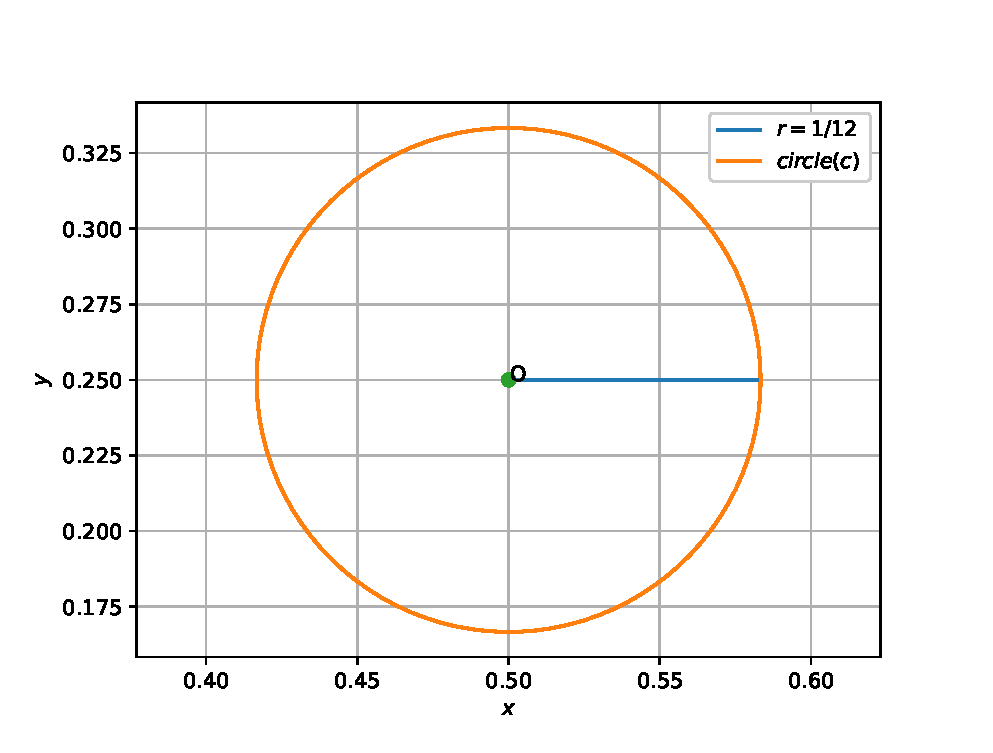
\includegraphics[width=\columnwidth]{./codes/circle2/pyfigs/circle2c.eps}
\caption{Circle with centre at $\myvec{\frac{1}{2}\\\frac{1}{4}}$ and radius $\frac{1}{12}$}
\label{fig:circle2c}
\end{figure}


\item
\begin{align}
\brak{d}\vec{O}=\myvec{1\\1}, r=\sqrt{2}
\label{eq:circle2d}
\end{align}
The following code sketches the circle \ref{eq:circle2d} in figure \ref{fig:circle2d} using the equation \ref{eq:eqn_of_circle}
\begin{lstlisting}
codes/circle2/circle2d.py
\end{lstlisting}
\begin{figure}[!ht]
\centering
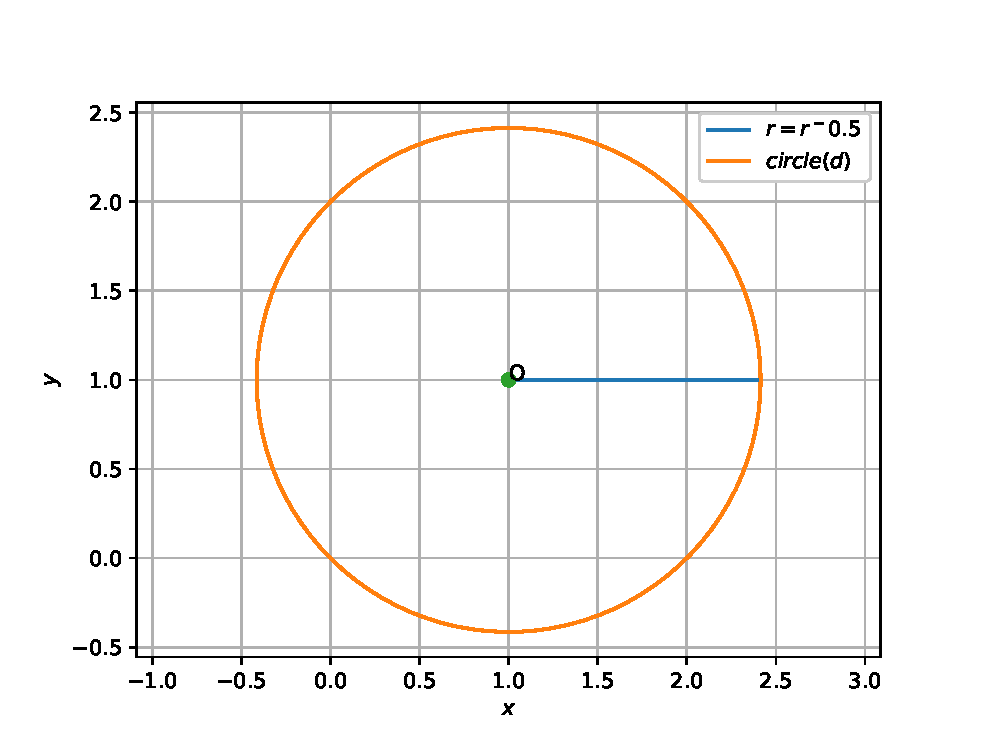
\includegraphics[width=\columnwidth]{./codes/circle2/pyfigs/circle2d.eps}
\caption{Circle with centre at $\myvec{1\\1}$ and radius $\sqrt{2}$}
\label{fig:circle2d}
\end{figure}

\item
\begin{align}
\brak{e}\vec{O}=\myvec{-a\\-b}, r=\sqrt{a^2-b^2}
\label{eq:circle2e}
\end{align}
The parameters used to sketch the circle are taken as 
\begin{align}
a=5,b=4
\implies \vec{O}=\myvec{-5\\-4}
\\
r=\sqrt{5^2-4^2}=3
\label{eq:circle2e_values}
\end{align}
The following code sketches the circle \ref{eq:circle2e_values} in figure \ref{fig:circle2e} using the equation \ref{eq:eqn_of_circle}
\begin{lstlisting}
codes/circle2/circle2e.py
\end{lstlisting}
\begin{figure}[!ht]
\centering
\includegraphics[width=\columnwidth]{./codes/circle2/pyfigs/circle2e.eps}
\caption{Circle with centre at $\myvec{-5\\-4}$ and radius $3$}
\label{fig:circle2e}
\end{figure}



\end{enumerate}
